\section{Designer}
\label{verwendung_designer}

\subsection{Neues Projekt erstellen}
\label{neuesprojekt}
Wenn Sie ein neues Spielentwickeln wollen, so sollten sie zunächst ein Projekt mit dem Designer erstellen. Wenn bereits ein Projekt erstellt wurde, können Sie zu \cref{projektladen} springen. (Siehe \cref{createprojekt})
Natürlich ist der Designer optional und Sie können ein Spiel vollkommen ohne ihn erstellen (Informationen zu der Syntax finden sie in der Doxygen Dokumentation, welche sich im Anhang befindet und in \cref{verwendung_engine}).
Um nun ein Projekt zu erstellen starten Sie den FM3D-Designer. Es öffnet sich nun ein Start-Layout (Siehe \cref{startlayout}). Klicken Sie nun auf die Schaltfläche \textit{New Project}. 
Daraufhin wird sich ein weiterer Dialog öffnen, in dem Sie nun den Namen und Pfad ihres Projektes angeben können. Durch die Schaltfläche \textit{Search} wird ein Explorer-Dialog geöffnet, in dem sie ihre Ordnerstruktur nach einem geeigneten Pfad durchsuchen können. Wenn Sie nun ihre Einstellungen getätigt haben, drücken Sie auf die Schaltfläche \textit{Start To Develope}. Sie werden nun auf den Haupt-Arbeitsplatz des FM3D-Designers weitergeleitet.
\begin{figure}
	\begin{center}
		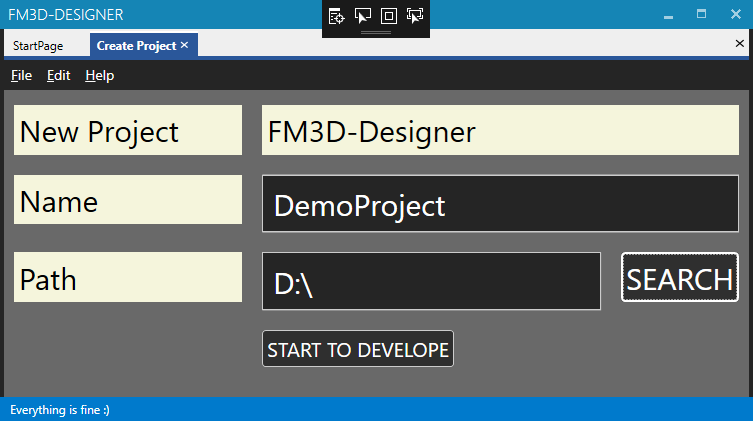
\includegraphics[width=0.5\textwidth]{04verwendung/Designer/00createproject.PNG}.
		\caption{Create-Dialog}\label{createprojekt}
	\end{center}
\end{figure}

\subsection{Altes Projekt laden}
\label{projektladen}
Falls Sie nun ein Projekt erstellt haben und es laden wollen, drücken Sie auf die Schaltfläche \textit{Load} rechts neben der Textbox. Es öffnet sich nun ein Explorer-Dialog in dem Sie nun eine \textit{.fmproj} Datei auswählen können. Wenn Sie nun eine Solche ausgewählt haben, drücken Sie auf \textit{Start}. Sie werden nun auf den Haupt-Arbeitsplatz des FM3D-Designers weitergeleitet.
Der Pfad des letzten geladenen Projektes kann durch den ContextMenü Punkt \textit{Last Project} in die Pfadleiste geladen und kann sofort geöffnet werden.

\subsection{Hauptarbeitsplatz}
Wenn sie nun in das Main-Layout (Siehe \cref{mainlayout}) gelangt sind befindet sich rechts ein File-Browser (Siehe \cref{filebrowser}). In diesem werden ihnen nun drei Ordner angezeigt. In diesen können Sie nun beliebig viele Entities erstellen und Ressourcen in das Projekt laden. Öffnen Sie nun ein Entity um verschiedene Komponente hinzuzufügen.
Auch können Sie Textdateien mit jeder beliebigen Endung zum Projekt hinzufügen.
Die Exportierten Ressourcen müssen Sie manuell in das Cpp Projekt einbinden.
Wenn Sie weitere Ordner in das Projekt einfügen wollen, speichern sie zunächst das Projekt ab und schließen Sie den FM3D-Designer. Gehen Sie dann in ihren Dateiexplorer, öffnen sie den Projektpfad und erstellen Sie an der beliebigen Stelle ein Verzeichnis. Laden Sie das Projekt neu über den Designer und klicken Sie mit der rechten Maustaste auf das Projekt-Item (Siehe \cref{item}). Ein \textit{ContextMenü} öffnet sich nun. Betätigen Sie den Schalter \textit{Include} und die Datei wird zum Projekt hinzugefügt.
\begin{figure}
	\begin{center}
		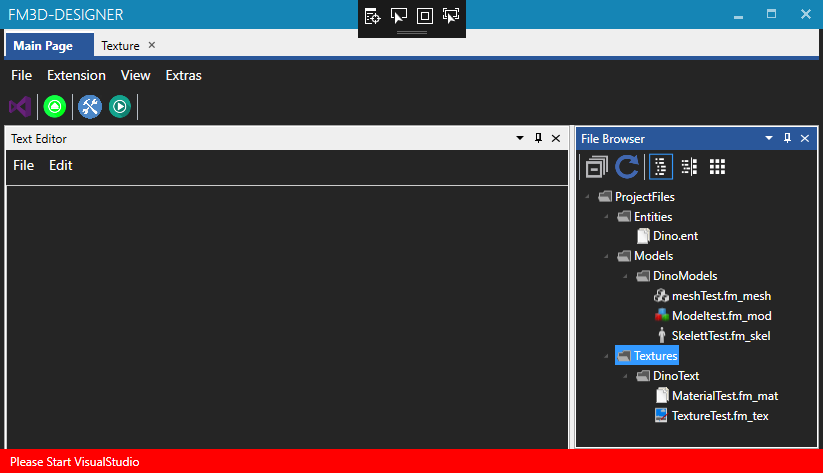
\includegraphics[width=0.5\textwidth]{04verwendung/Designer/01workstation.PNG}
		\caption{Haupt-Fenster des FM3D-Designers}\label{arbeitsplatz}
	\end{center}
\end{figure}

\subsection{Extension}
Stellen Sie sicher, dass die FM3D-Extension installiert ist und starten sie darauf hin das VisualStudio-Projekt aus dem Designer. Klicken Sie, falls Sie es nicht schon getan haben, hierfür auf das Visual-Studio Icon im Designer. ([1] in \cref{extmen})
Bestätigen Sie die \textit{MessageBox} und warten Sie bis das Projekt geladen wurde.
Wenn es nun geladen wurde, überprüfen Sie nochmal ihre Entities im File-Browser. Falls alle ihren Vorstellungen übereinstimmen, gehen Sie nun auf den zweiten Schalter und betätigen Sie diesen. ([2] in \cref{extmen})
Nun werden die Entity-Preset Klassen in dem VisualStudio-Projekt generiert. Speichern Sie ihr Projekt anschließend.
Wenn sie ihr Spiel fertig Programmiert haben, so können Sie es über das Programm mit den zwei letzten Icons Debugen und Compilen ([3] und [4] in \cref{extmen}), falls Sie noch gerade im Designer beschäftigt sind. Diese Funktion ist optional.
\begin{figure}
	\begin{center}
		
\includegraphics[width=0.2\textwidth]{04verwendung/Designer/02ExtensionMenu.PNG}.
		\caption{Extension Menü}\label{extmen}
	\end{center}
\end{figure}